\subsection{Characterization of Performance}

\subsubsection{A. Experiment Setup}

We perform scalability experiments on Blue Waters HPC resource-- a 13.3 petaFLOPS Cray at NCSA and University of Illinois, with 32 Interlago cores/50 GB RAM per node, Cray Gemini, Lustre shared file system. 

We characterize the weak scalability of the ESMACS protocol HT-BAC workflow using Ensemble Toolkit. We ran the HTBAC workflow with null workloads where the task did no work (/bin/sleep 0), and NAMD workload launched using MPI. The size of the workload is varied in proportion with the amount of resources such that all tasks are concurrently executed at all times. The number of replicas ranged from 8 to 128 running concurrently using 8 cores per replica. Stages 4 and 6 are assigned 5000 steps while stage 5 requires 55000 steps. 

\subsubsection{B. Results}

We perform weak scalability characterization of HTBAC for both null workload and NAMD workload by measuring the overhead introduced by RP and the simulation execution time. The RP overhead demonstrates the core overhead which is the time-to-completion (TTC) as measured by RADICAL Pilot as well as the Blue Waters file system overhead, network communication, and time to stage the units. For the NAMD workload, figure Y shows scalability results for the overheads and the simulation execution time which corresponds to the time taken by all the simulations to complete. All the experiments use Ensemble Toolkit version 0.47. 

\begin{figure}[!htbp]
  \centering
  \begin{minipage}[b]{0.49\textwidth}
  \centering
  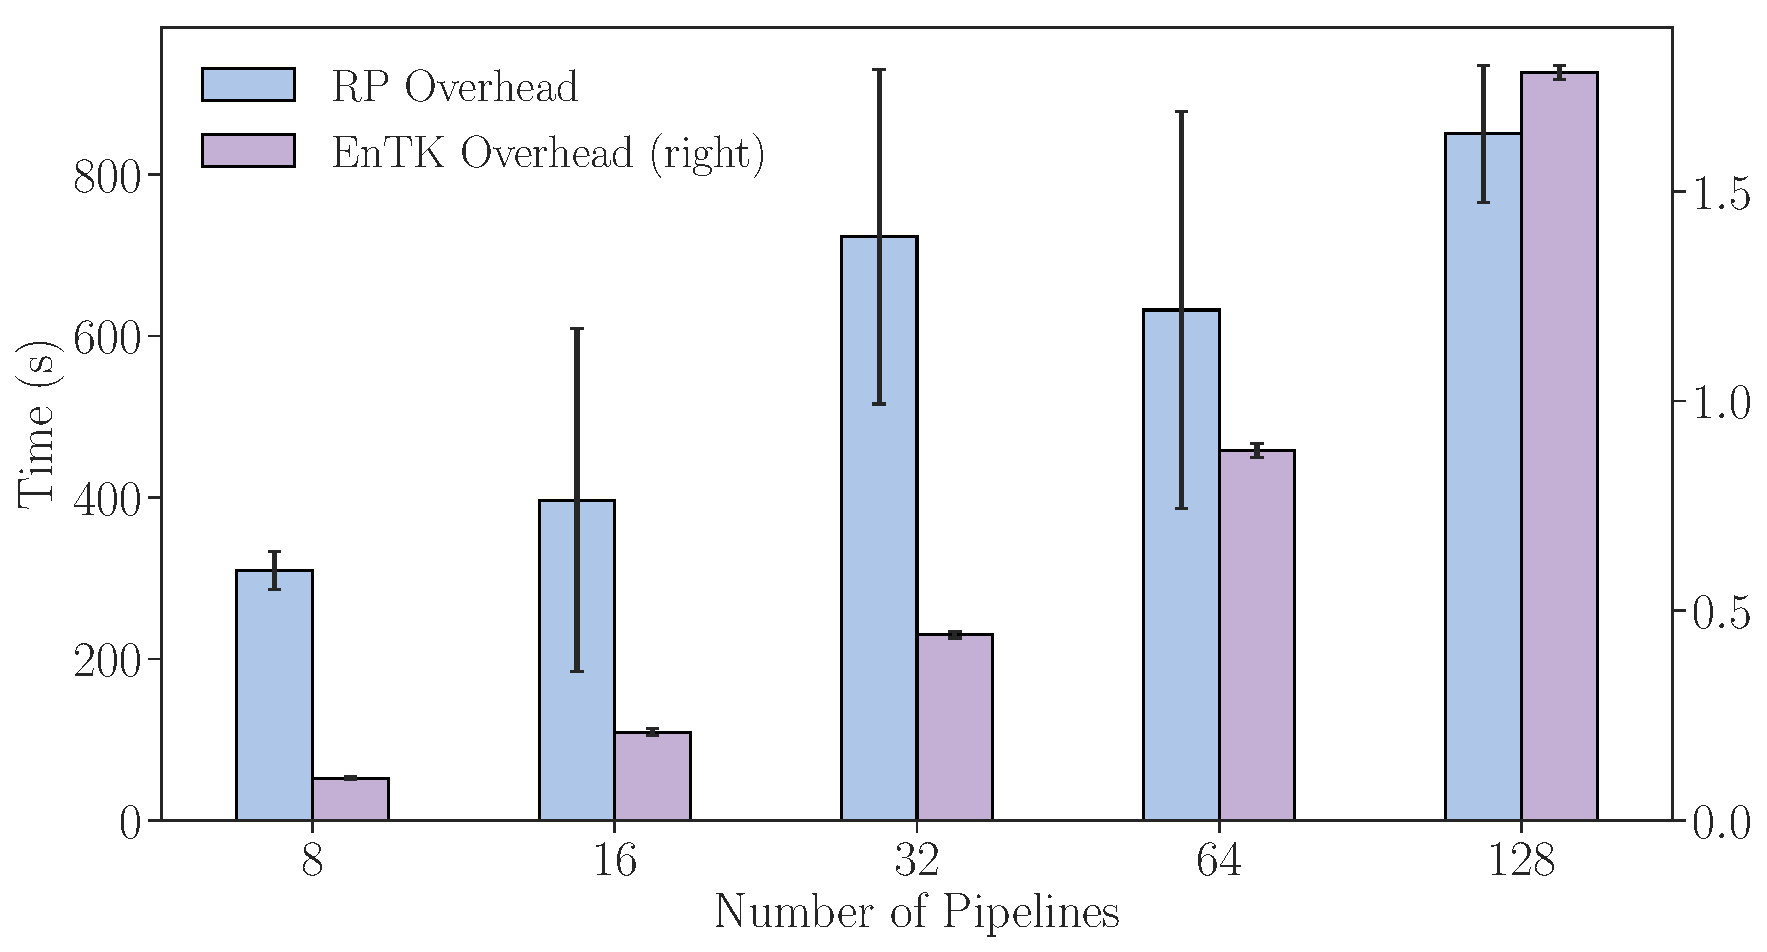
\includegraphics[width=\textwidth]{FIGURES/null_workload_overheads.pdf}
  \end{minipage}
  \begin{minipage}[b]{0.49\textwidth}
  \centering
  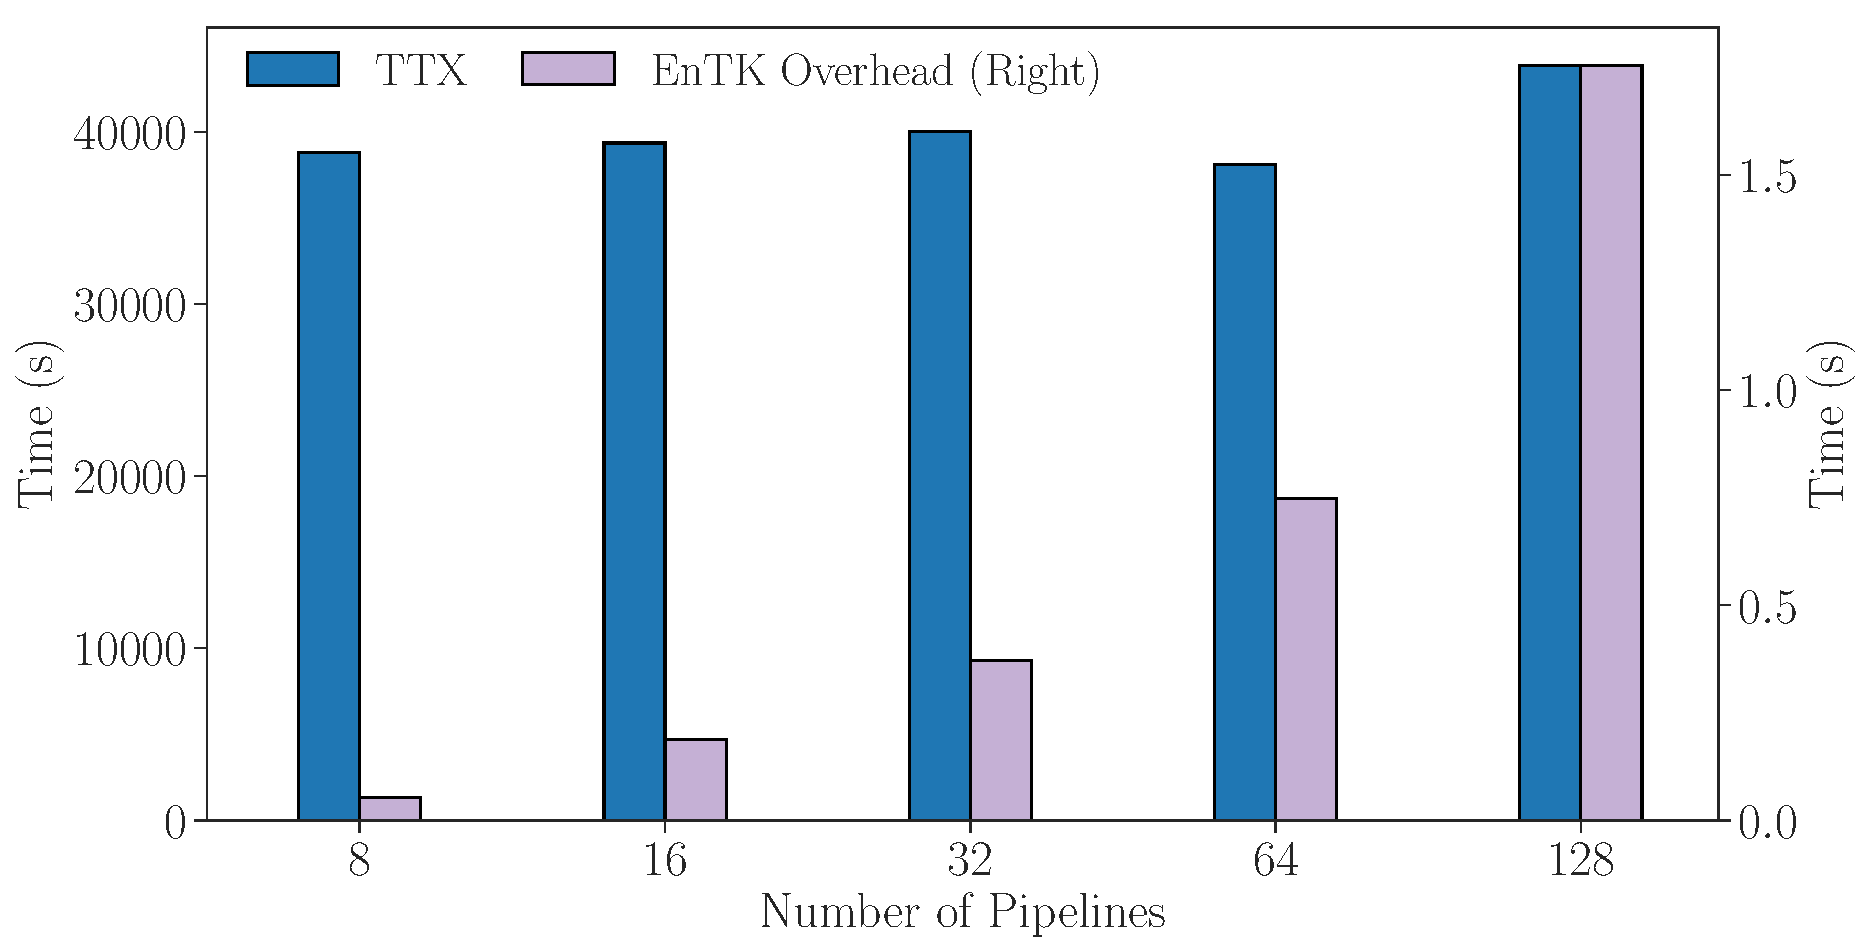
\includegraphics[width=\textwidth]{FIGURES/namd_workload_overheads.pdf}
  \end{minipage}

\caption{\textbf{Left:} Weak scaling of HTBAC using null workload. We observe
similar behavior at each configuration in the simulation execution time
showing that the RADICAL-Pilot is invariant to the workload and a steady
increase in the RP overhead due to the increase in the number of stages.
\textbf{Right:} Weak scaling of HTBAC using NAMD workload. We observe higher
simulation execution times than the null workload yet similar behaviour in
all NAMD configurations.}\label{fig:htbac_perf}
\end{figure}


The fluctuation of the simulation execution times can be attributed to run-time system fluctuations within the workload including stragglers at higher pipeline and pipeline-to-pipeline fluctuations. In order to examine the fluctuations within stages we corrolate the overhead for each pipeline at the longest simulation duration in order to reconcile any fluctuations induced by NAMD. We calculate time-to-execution (Tx) of the largest pipeline size and compare the longest MD run within each pipeline. The NAMD logs indicate a mean and variance as ...

\begin{figure}[!htbp]
  \centering
  %\begin{minipage}[b]{0.6\textwidth}
  \begin{minipage}[b]{0.55\textwidth}
  \centering
  %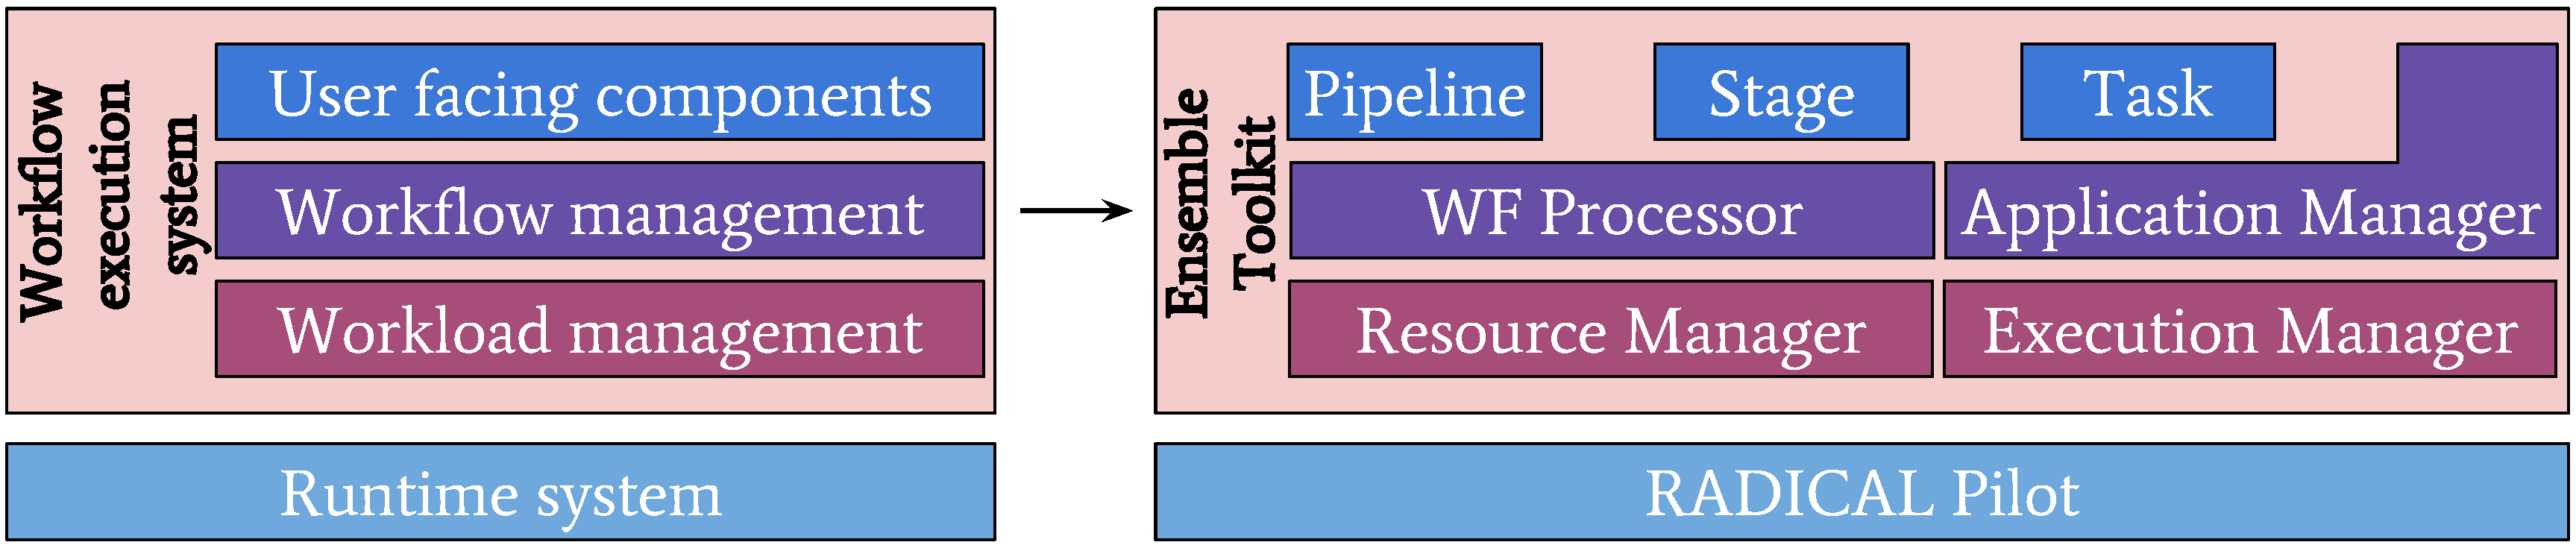
\includegraphics[width=\textwidth, height=35mm]{FIGURES/entk_overview.pdf}
%  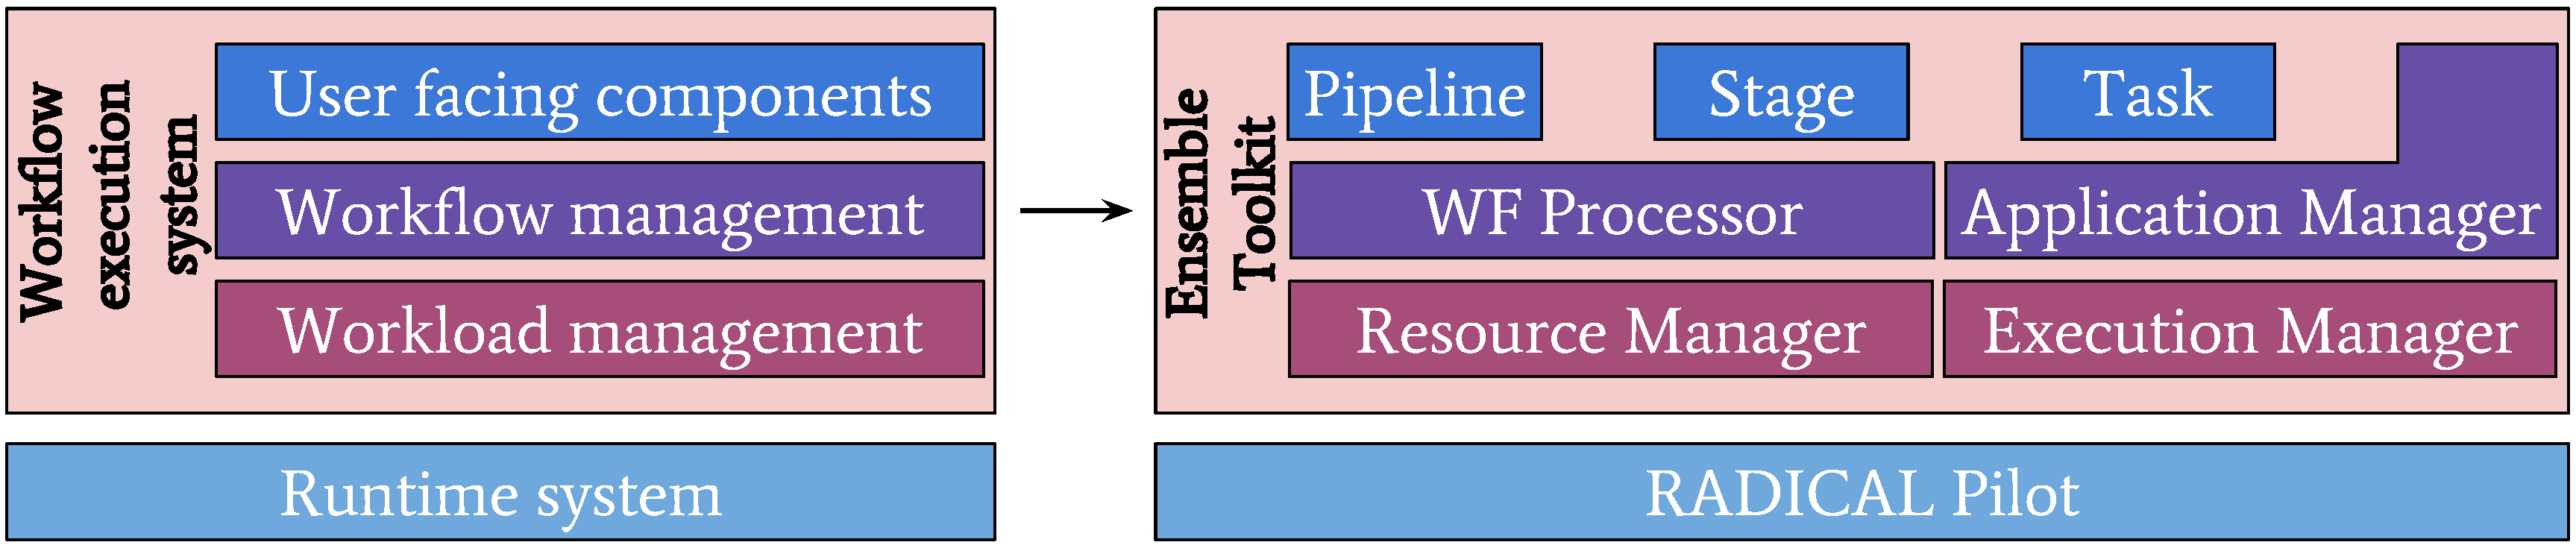
\includegraphics[width=\textwidth, height=40mm]{FIGURES/entk_overview.pdf}
  \end{minipage}
  %\begin{minipage}[b]{0.39\textwidth}
  \begin{minipage}[b]{0.44\textwidth}
  \centering
%  \includegraphics[width=\textwidth, height=35mm]{FIGURES/md_general.pdf}
%  \includegraphics[width=\textwidth, height=40mm]{FIGURES/md_general.pdf}
  \end{minipage}
\caption{Overview of time-to-execution (Tx) of each pipeline at the longest simulation duration as measured by NAMD log files, showing how the distribution shows no abnormal fluctuations across pipelines.}
\label{fig:namd_logs}
\end{figure}

%NAMD logs - corrolate the overhead for each pipeline makes the system invariant to the worload. Remaining will be RP overhead. NAMD log files (utime) demonstrates time-to-execution (Tx) 

%Add in: what are the overheads, how is EnTK collecting overhead 

The use-case only requires up to 25 replicas which we demonstrate is more than sufficient. 


%eq0 : Minimize with decreasing restraints
%eq1 : NVT, 50K, with restraints
%eq2 : NPT, 300K, with decreasing restraints 
%sim1.conf: NPT, 300k, no constraints


Need system verification of timestamps (errors) 




